It is important that any image is fed into the network crop by crop, meaning that for each crop there is a separate embedding. In this section crops embeddings were not combined in any way together and were analysed separately.

The UNet embedding has a size of $16 \times 16 \times 256$ and can be flattened into a $655536$-dimensional vector. In order to comprehend the embeddings for us as humans, a dimensionality reduction algorithm has to be applied. One option would be to compress a vector to 2D or 3D representation, which is easily comprehendable by humans.
\begin{figure}[htb]
	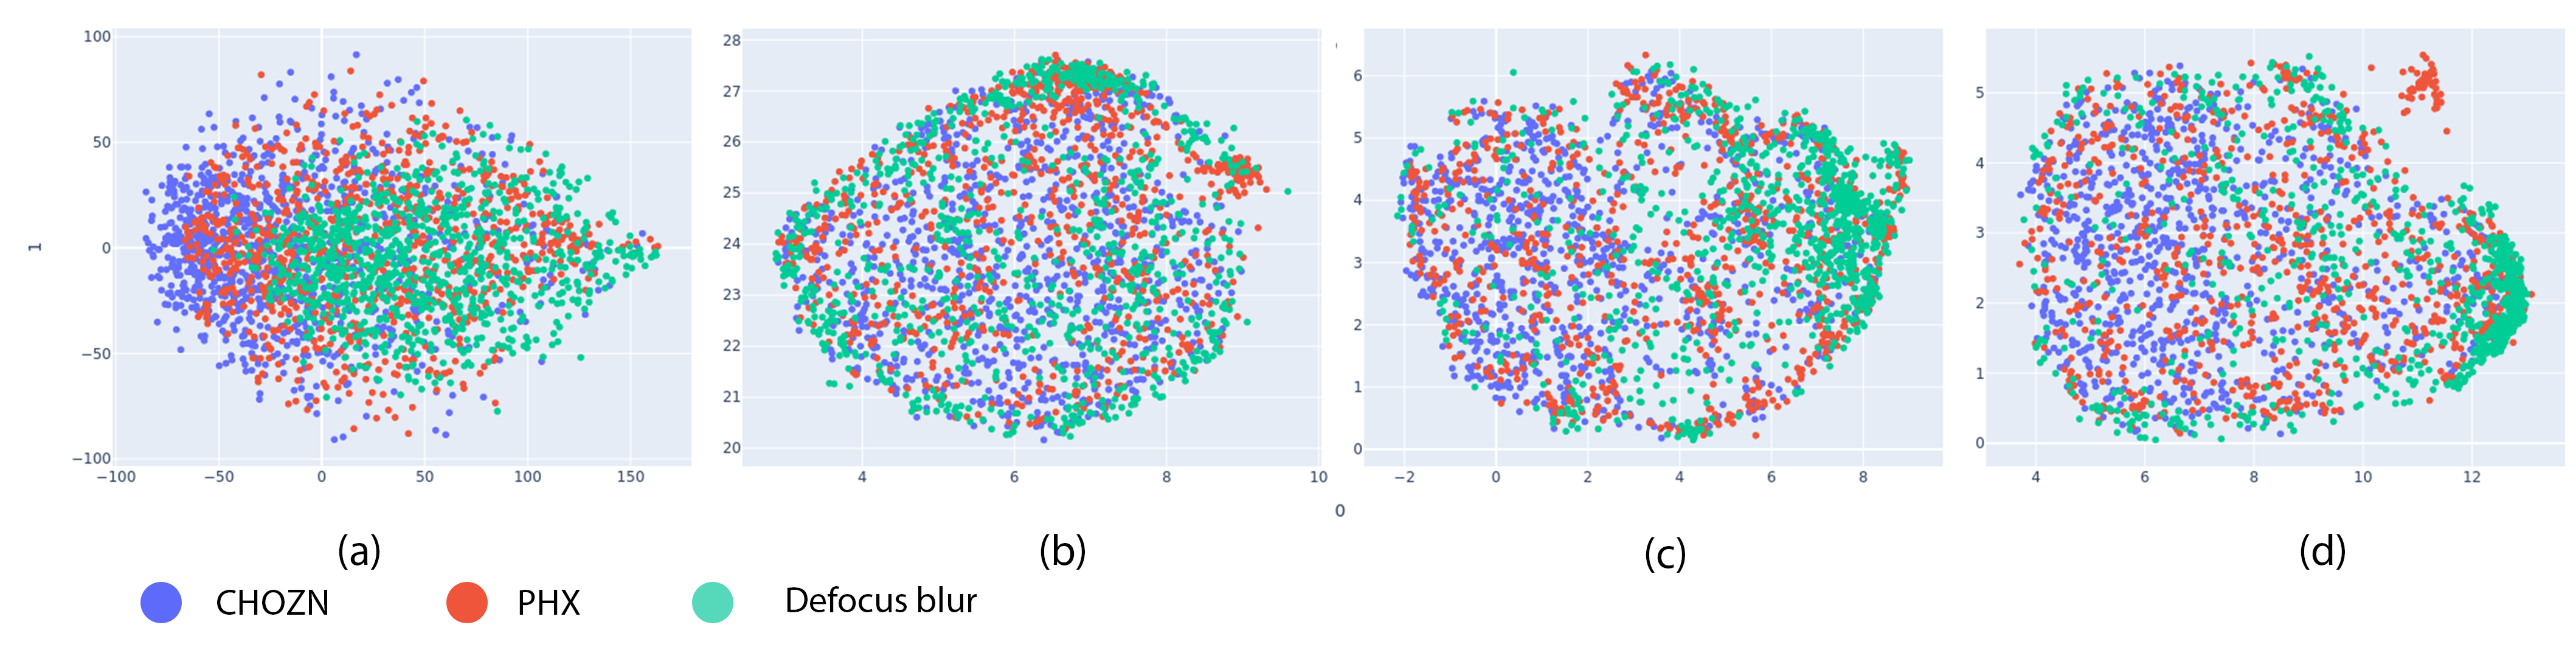
\includegraphics[width=\linewidth]{bilder/unet-embeddings/umap-pca-embeddings.png}
	\caption[Visualization of UNet embeddings in 2D space]%
	{Visualization of UNet embeddings in 2D space. (a) PCA, (b) UMAP, (c) combination of PCA and UMAP with 10 and (d) 200 components. First row differentiates between two cell phenotypes: CHOZN and PHX, whereas the second row differentiates between uncorrupted crops and crops corrupted using artificial defocus blur of severity level $4$.}\label{fig:umap-pca-embeddings}
\end{figure}

In this case a two-dimensional representation was chosen. With the help of PCA, UMAP and their combination embeddings were projected into a 2D space. In Figure \ref{fig:umap-pca-embeddings} we can see kernel density estimate (KDE) plots, that were created based on scatter plots, where each dot represents a projected UNet embedding of a crop. Both research questions are addressed here: clustering based on phenotypes (CHOZN or PHX) and clustering based on input corruptions (defocus blur of severity level $4$). It is crucial here that corrupted data was not used in training of any of dimensionality reduction method. The goal was to use only the data available in training dataset, find the transformation of high-dimensional data into a lower-dimensional space and apply it to new samples. That is also why methods like t-sne (\cite{t-sne}) cannot be used here, because the transformation that t-sne learns cannot be applied to new samples. 

From Figure \ref{fig:umap-pca-embeddings} it becomes evident that there is no clustering based on the phenotype. On the one hand, this means that it is not possible to detect phenotype based on the UNet embedding. But on the other hand, this also implies that PHX or CHOZN phenotypes do not influence the predictions so much supports previous conclusion from Section \ref{section:generalizability-across-phenotypes} that the model generalises well across them. Regarding the clustering based on the artificial corruption it seems that embeddings of corrupted samples tend to clump more in groups, occupying one specific area of the embeddings space. It is also clear that the combination of UMAP with previously applied PCA works better with the increasing amount of components in PCA: dots in (d) seem to form a better cluster than dots in (c). However, it can still not be taken intuitively from this figure how many non-corrupted dots are hidden behind the cluster of the green dots --- meaning whether non-corrupted crops cluster intersects severely with a corrupted one. In order to visualize this better, one can use a kernel density estimate (KDE) plot presented in Figure \ref{fig:kde}. Additionally, it is clear that pure UMAP is not the best approach for the extreme number of dimensions as with the one in this case.

%\begin{figure}[htb]
%	\begin{center}
%		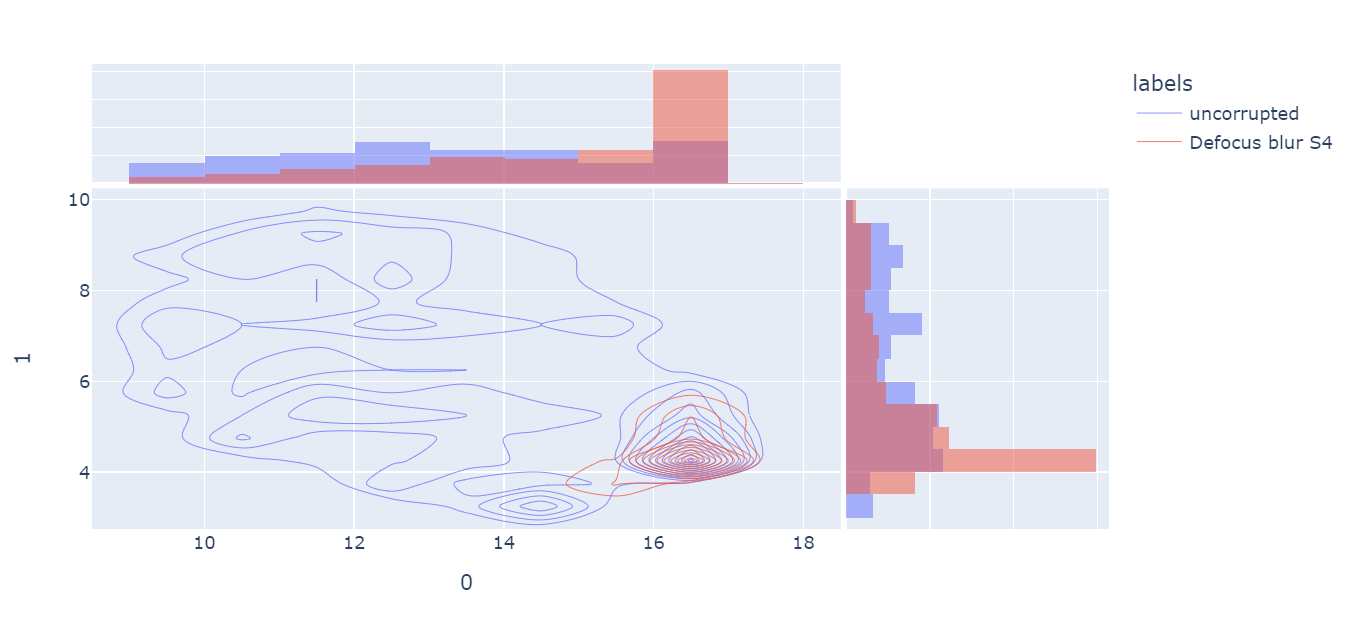
\includegraphics[width=0.6\linewidth]{bilder/unet-embeddings/kde.png}
%	\caption{KDE plot of UMAP applied after PCA with 200 components}\label{fig:kde}
%	\end{center}
%\end{figure}

A cluster of corrupted images is clearly present here, however it also intersects with many non-corrupted crops. The quantitative evaluation of how this cluster is separable from the rest of the points is provided in section \ref{section:clustering-on-unet-embeddings}. Although one can already state that there is a clear opportunity to differentiate between corrupted and not corrupted images, the accuracy cannot be high due to the clusters being not well separable. For further research it is suggested to additionally check whether clusters form into a high-dimensional space before projecting them into a 2D space. 

\paragraph{Clustering with PaCMAP}
\label{section:clustering-on-unet-embeddings}
Since the UNet embeddgins are the most promising for clustering based on input corruptions we will proceed with this approach. Apart from dimensionality reduction methods used in section \ref{section:unet-embeddings-dim-reduction}, PaCMAP clustering was tried. You can find its detailed description in section \ref{section:pacmap}. 
\begin{figure}[htb]
	\begin{center}
		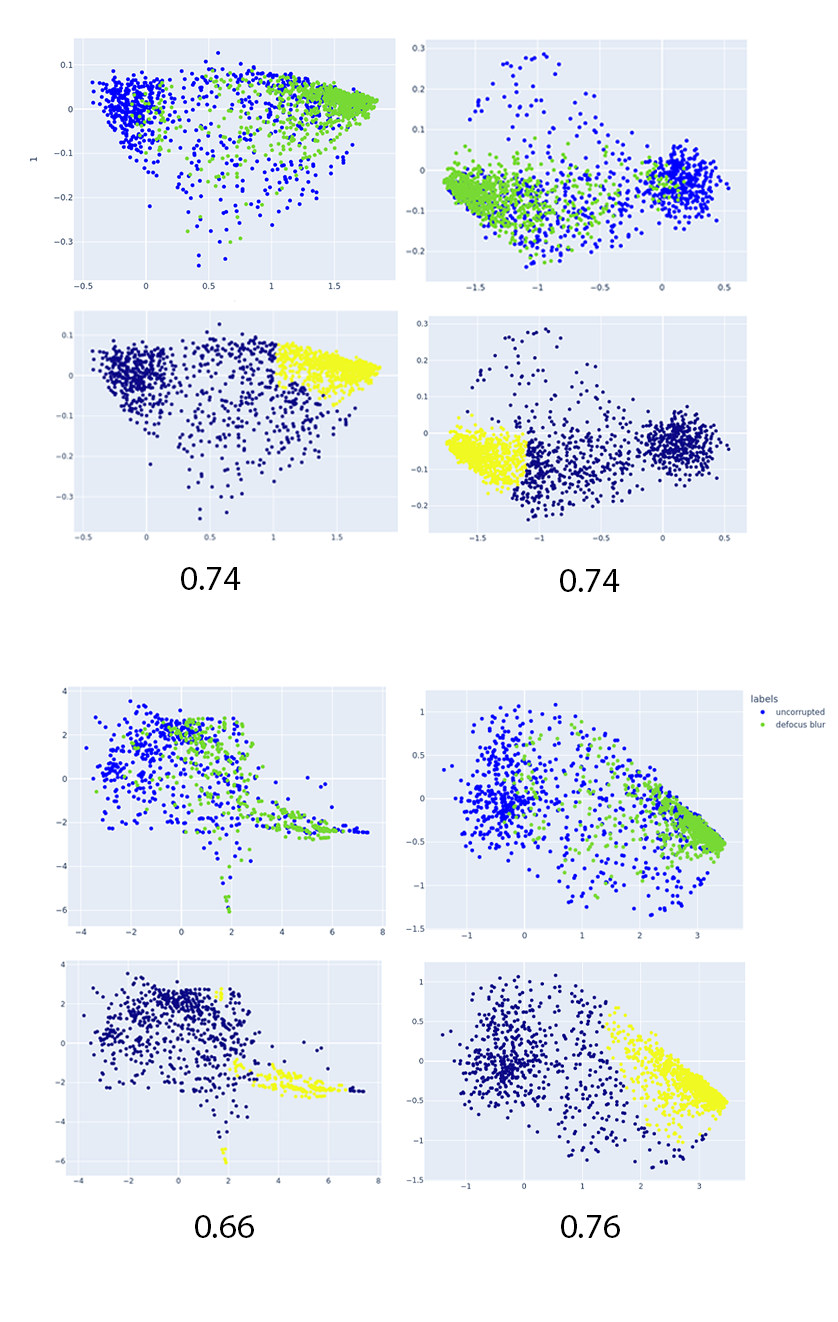
\includegraphics[width=\linewidth]{bilder/unet-embeddings/PacMAP.png}
		\caption{Clustering of UNet embeddings after PacMAP}
		\label{fig:unet-clustering}
	\end{center}
\end{figure}

PaCMAP allows a more flexible hyperparameter tuning in order to preserve local and global relations from high-dimentional data and as result a better clustering can be found. As usual PaCMAP was trained using "good" training data only, meaning no corruptions were introduced. And only when the transformation from high-dimensional into a lower dimensional space was found, corrupted crops were projected using this transformation. Figure \ref{fig:unet-clustering} presents results of training PaCMAP with 4 different hyperparametrization settings. There are 3 hyperparameters that were changed here: MN\_ratio, FP\_ratio and n\_neighbors. Detailed explanation of their influence was also described in section \ref{section:pacmap}. From left to right in Figure \ref{fig:unet-clustering}:

\begin{itemize}
	\item MN\_ratio=0.5, FP\_ratio=0.1, n\_neighbors=10
	\item MN\_ratio=0.1, FP\_ratio=0.1, n\_neighbors=10
	\item MN\_ratio=0.5, FP\_ratio=0.5, n\_neighbors=2
	\item MN\_ratio=0.1, FP\_ratio=0.5, n\_neighbors=10
\end{itemize}

In this case cluster of green dots represents projected UNet embeddings of images corrupted with defocus blur with severity level $4$, which is already a strong corruption and leads to unacceptable predictions of the model, that did not have defocus blur augmentations. However, these point are still strongly mixed with not corrupted ones. In order to check how separable they are unsupervised clustering DBSCAN alogorithm was used. Results of this clustering are shown in Figure \ref{fig:unet-clustering-sev-levels}. Density based clustering approach used here was described in details in section \ref{section:dbscan}. 

\begin{figure}[htb]
	\begin{center}
		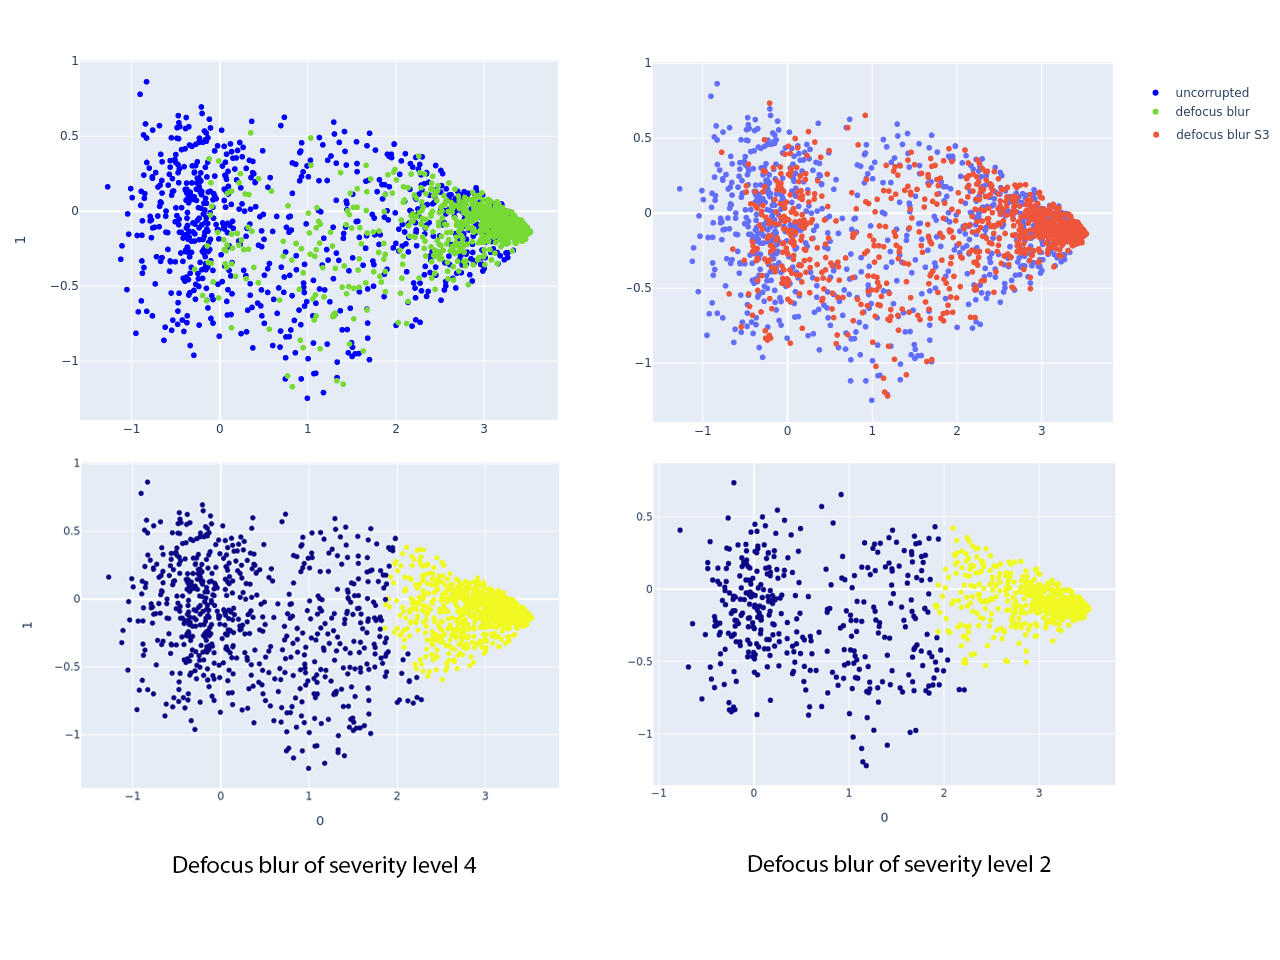
\includegraphics[width=0.6\linewidth]{bilder/unet-embeddings/db-levels.png}
		\caption{Clustering of UNet embeddings after PacMAP for different severities levels}
		\label{fig:unet-clustering-sev-levels}
	\end{center}
\end{figure}

After training DBSCAN on not corrupted crops embeddings it has recognized a class on the right (yellow dots) as a cluster and the rest of the points (blue ones) as noise, because they have quite low density in comparison to the yellow cluster. This is not a problem if we consider noisy points simply as a separate cluster. For such clustering defocus blur of level $4$ splits the crops between two clusters with an F1-score of $0.74$. In Figure \ref{fig:unet-clustering-sev-levels} on the right red points represent projection of image embeddings after corrupting them with a defocus blur of severity level $3$. In this case they are mixed with not corrupted projections even stronger. Here prediction of already trained DBSCAN drops to F1-score of $0.64$.

Overall UNet embeddings do express clustering of corrupted embeddings to a small extent, however not strongly enough to use it in practice. Autoencoder here would be a better approach, however brightness normalization has to take place first. It is recommended to proceed the research here in the direction of contrastive learning algorithms, specifically \cite{csi} approach.
